\begin{figure}[thb]
  \begin{center}
    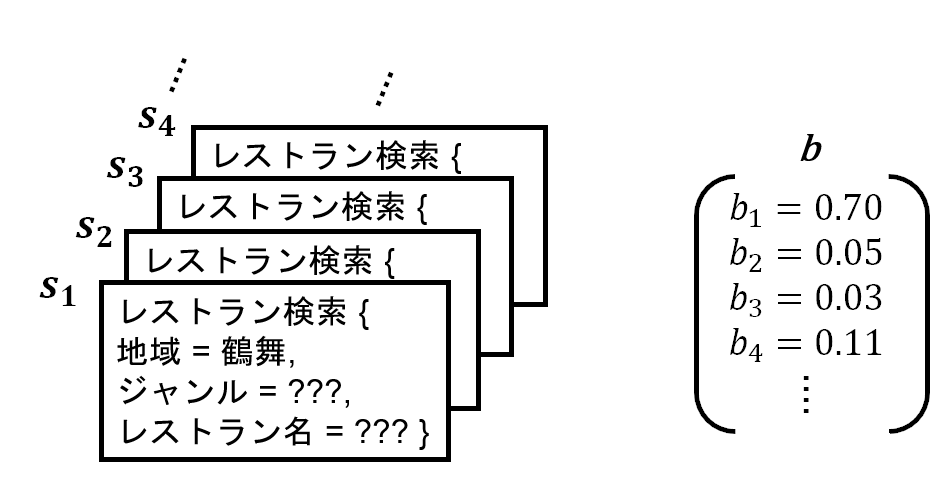
\includegraphics[width=10cm]{chapter2/belief.eps}
    \caption{信念}
    \label{fig:belief}
  \end{center}
\end{figure}

\begin{figure}[thb]
  \begin{center}
    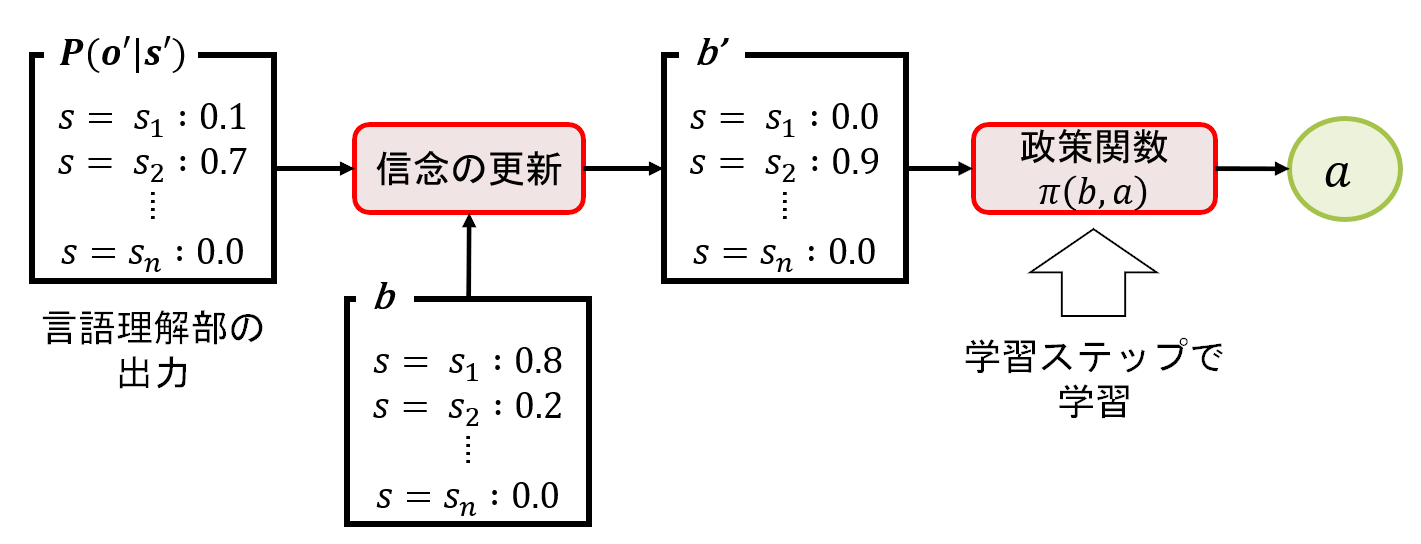
\includegraphics[width=15cm]{chapter2/pomdp2.eps}
    \caption{部分観測マルコフ決定過程(POMDP)の流れ}
    \label{fig:pomdp}
  \end{center}
\end{figure}

統計的機械学習による対話状態追跡では,言語理解部からの誤りに対する頑健性を得るために,対話状態を確率的に扱う.これは,ユーザ発話の解釈に不確実性が存在するため,対話状態を直接観測できないとしているからである.対話状態の確率的表現は,全ての対話状態にわたる確率分布である信念 $b$ を用いる.信念に関する図を図\ref{fig:belief}に示す.また,言語理解部の出力はノイズを含むユーザ入力の観測 $o$ とする.対話状態の推定は,ターン $t$ の対話状態を $s^t \in I_s$,
システムの行動を $a^t \in K$,観測状態を $o^t \in I_s$,ユーザの対話状態が$s$である信念(確率変数)を $b^t_s$ として,式\ref{joutai_suitei}を推定する問題となる.
\begin{equation}
  \label{joutai_suitei}
  b_s = P(s|o^{1:t})
\end{equation}
$P(s|o^{1:t})$ は,これまでの観測状態から推定した全てのユーザの対話状態にわたる確率分布である.つまり,履歴としてこれまでの観測状態を用いている.
\par
統計的機械学習による対話管理の一例として,部分観測マルコフ決定過程(Partially Observable Markov Decision Process ; POMDP)\cite{pomdp,pomdp_review}を用いた手法を説明する.POMDPベースのモデルは,信念状態の追跡と強化学習という2つのキーアイデアを組み合わせている.\cite{pomdp_review}
\par
POMDPでは図\ref{fig:pomdp}のように,言語理解部の出力を全ての対話状態にわたる確率分布 $p(o'|s')$ で表す.そして,信念状態の追跡には対話状態を最新の対話状態に更新する状態更新関数を用いる.状態更新関数は現在の対話状態 $s^{t+1}$ をこれまでの観測状態系列 $o^{1:t+1}$ から求める式である.状態更新関数は式\ref{state_update}に示す.
\begin{equation}
  \label{state_update}
  b' = P\left(s^{t+1}|o^{1:t+1}\right) \propto P\left(o'|s'_{j}\right) \Sigma_{s_i} P\left(s'_{j}|s_i, \widehat{a_k}\right)b^t
\end{equation}
式\ref{state_update} では,$P(o'|s'_j)$が観測確率,$P(s'_j|s_i,\widehat{a_k})$ が状態遷移確率,$b_t$が現在の信念を表す.
\par
信念の更新をした後,状態 $s$ で対話行為 $a$ を選ぶ確率である政策関数$\pi (b,a)$を用いて次のシステムの対話行為を決める.POMDP では信念と対話行為から報酬を計算し,政策関数を強化学習により最適化していく.報酬には 状態行動価値(Q値)などを用いる.Q 値とは,ある状態 $s$ の時 対話行為 $a$ を行い得られる報酬の期待値 $R_E(s,a)$ である.そして,行動価値関数 $Q^{\pi}(s,a)$ を最大化する政策関数 $\pi^{*}$を選択する.行動価値関数は式\ref{qkansu}に示す.$\gamma$ は忘却率とする.
\begin{eqnarray}
  Q^{\pi}(s,a) & = & \sum^{\infty}_{k=0} \gamma^k R_E\left(s^{t+k},a^{t+k}\right) \\
  & = & \sum_{s^{t+1}}P\left(s^{t+1}|s^t,a^t\right)\left(R\left(s^t,a^t,s^{t+1}\right) + \gamma\sum^{\infty}_{k=0} \gamma^k R_E\left(s^{t+k+1},a^{t+k+1}\right)\right) \\
  \label{qkansu}
  & = & \sum_{s^{t+1}}P\left(s^{t+1}|s^t,a^t \right) \left(R\left(s^t,a^t,s^{t+1}\right) + Q^{\pi}\left(s^{t+1},a^{t+1}\right)\right)
\end{eqnarray}
次に,Q 学習によって Q 値の更新を繰り返し収束させる.Q値の更新は式\ref{qupdate}で行う.$\alpha$ は学習率とする.
\begin{eqnarray}
  \label{qupdate}
  Q\left(s^t,a^t\right) \xleftarrow[update]{} \left(1-\alpha\right)Q\left(s^t,a^t\right) + \alpha \left(R\left(s^t,a^t,s^{t+1}\right) + \gamma \max_{a^{t+1}}Q\left(s^{t+1},a^{t+1}\right)\right)
\end{eqnarray}
$R(s^t,a^t,s^{t+1})$ は $s^t$ の時 $a^t$ を行い $s^{t+1}$ に遷移したときの報酬を表す.Q 学習によって報酬が決まった後,その報酬を用いて政策関数の学習を行い,最適な対話行為を選ぶことを目指すのがPOMDP を用いた対話管理である.
\par
POMDP の問題には,複雑なタスクや複数のタスクを取り扱うと対話状態のパターンが増加するため,信念の計算量が膨大になること,ルールベースほどではないが言語理解部以前の誤りから悪影響を受けることなどが挙げられる.